\documentclass[a4paper,twoside]{llncs}

\usepackage{url}
\usepackage{graphicx}
\usepackage{inconsolata}
\usepackage{listings}
%\usepackage{caption}[2015/09/20]
\usepackage{enumitem}
\usepackage[T1]{fontenc}
\usepackage[utf8]{inputenc}
\usepackage{xcolor}
\usepackage{xspace}
\usepackage{epsfig}
\usepackage{subfigure}
\usepackage{calc}
%\usepackage{amssymb}
%\usepackage{amstext}
%\usepackage{amsmath}
%\usepackage{amsthm}
\usepackage{multicol}
\usepackage{pslatex}
\usepackage{apalike}
%\usepackage{SCITEPRESS}     % Please add other packages that you may need BEFORE the SCITEPRESS.sty package.

\subfigtopskip=0pt
\subfigcapskip=0pt
\subfigbottomskip=0pt


\graphicspath{{../img/}}

\definecolor{myblue}{HTML}{406E86}
\definecolor{codeblue}{HTML}{004385}
\definecolor{codegrey}{HTML}{4D4D4D}
\definecolor{rulerline}{HTML}{A0A2AC}
\definecolor{codegreen}{HTML}{518D71}
\definecolor{codeviolet}{HTML}{7F0055}
\definecolor{darkblue}{HTML}{08088A}
\definecolor{mygrey}{HTML}{4D4D4D}

\newcommand{\IOT}{IoT\xspace}
\newcommand{\IOTDSL}{\textsf{IoTD\scriptsize\MakeUppercase{sl}}\xspace}
\newcommand{\DSL}{\textsc{Dsl}\xspace}
\newcommand{\DSLS}{\textsc{Dsl}s\xspace}
\newcommand{\MDE}{\textsc{Mde}\xspace}
\newcommand{\CEP}{\textsc{Cep}\xspace}

%%%%%%%%%%%%%%%%%%%%%%%%%%%%%%%%%%%%%%%%%%%%%%%%%%%%%%%%%%%%%%%%%%%%%%%%%%
%%%%%%%%%%%%%%%%%%%%%%%%%%%%%%%%%%%%%%%%%%%%%%%%%%%%%%%%%%%%%%%%%%%%%%%%%%
%%%%%%%%%%%%%%%   TODO & COMMENTS

\usepackage{todonotes}

\newif\ifdraft\drafttrue
\ifdraft
   \newcommand\todos[1]{\medskip\todo[inline]{TODO (all): #1}}
   \newcommand\moussa[1]{\medskip\todo[color=green!40,inline]{TODO (Moussa): #1}}
   \newcommand\fabian[1]{\medskip\todo[color=purple!40,inline]{TODO (Fabian): #1}}
\else
   \newcommand\todos[1]{}
   \newcommand\moussa[1]{}
   \newcommand\fabian[1]{}
\fi
%%%%%%%%%%%%%%%%%%%%%%%%%%%%%%%%%%%%%%%%%%%%%%%%%%%%%%%%%%%%%%%%%%%%%%%%%%

%%%%%%%%%%%%%%%%%%%%%%%%%%%%%%%%%%%%%%%%%%%%%%%%%%%%%%%%%%%%%%%%%%%%%%%%%%
%%%%%%%%%%%%%%%%%%%%%%%%%%%%%%%%%%%%%%%%%%%%%%%%%%%%%%%%%%%%%%%%%%%%%%%%%%
%%% DSL Syntax Definition
%%%%%%%%%%%%%%%%%%%%%%%%%%%%%%%%%%%%%%%%%%%%%%%%%%%%%%%%%%%%%%%%%%%%%%%%%%

\lstdefinelanguage{iotdsl}{
  morecomment=[l]{//},
  morecomment=[s]{/*}{*/},
  morestring=[d]",
  morestring=[d]',
  morekeywords={
    configuration, node, from, to, via,
    sensing, actuating, gateway, device,
    rule, when, before, after, and, do, in, out, within, not, true, false
  }
}

\lstdefinelanguage{tesla}{
  morecomment=[l]{//},
  morecomment=[s]{/*}{*/},
  morestring=[d]",
  morestring=[d]',
  morekeywords={
    define, where, from, consuming, or, and, within, not, true, false, =, := 
  }
}

\lstset{
  basicstyle=\fontsize{7}{8}\ttfamily,
  basewidth={0.55em,0.45em},
  keywordstyle=\bfseries\color{codeviolet},
  commentstyle=\itshape\color{mygrey},
  stringstyle=\color{darkblue},
  identifierstyle=\mdseries\color{black},
  numbers=left,
  numberstyle=\tiny\color{rulerline},
  stepnumber=1, 
  numbersep=5pt,
  firstnumber=1, 
  frame=lines,
  rulecolor=\color{rulerline},
  tabsize=2,
  breaklines=true,
  aboveskip=4pt,
  belowskip=4pt,
  showspaces=false,
  showstringspaces=false,
  captionpos=b,
  literate={~} {$\sim$}{1},
  showlines=true
}

\def\inlineT{
	\lstinline[basicstyle=\ttfamily,language=tesla]
}

\def\inlineI{
	\lstinline[basicstyle=\ttfamily,language=iotdsl]
}

%%%%%%%%%%%%%%%%%%%%%%%%%%%%%%%%%%%%%%%%%%%%%%%%%%%%%%%%%%%%%%%%%%%%%%%%%%
%%%%%%%%%%%%%%%%%%%%%%%%%%%%%%%%%%%%%%%%%%%%%%%%%%%%%%%%%%%%%%%%%%%%%%%%%%


\begin{document}

\renewcommand{\thelstlisting}{\arabic{lstlisting}}

\title{Complex Event Processing for User-Centric Management of IoT Systems}
\author{Moussa Amrani\inst{1} \and Fabian Gilson\inst{1} \and Vincent Englebert\inst{1}}

\institute{
	University of Namur, PReCISE Research Center, Namur, Belgium\\
	\email{\{moussa.amrani, fabian.gilson, vincent.englebert\}@unamur.be}
}

\maketitle 

\begin{abstract}
	The amount of available connectible devices and Internet of Things (\IOT) solutions is increasing as such equipments are becoming popular and widely available on the market. This growth in popularity goes together with a keen interest for \textit{smart homes} where individuals deploy \textit{ad hoc} solutions in their houses. However, the task to translate the users' needs into a concrete \IOT infrastructure is not straightforward and often require to deal with proprietary APIs and technical details, so that the link to user requirements may be lost as well as the validity of their interaction properties can scarcely be verified. In order to define and manipulate devices deployed in domestic environments, we propose \IOTDSL, a Domain-Specific Language relying on a high-level rule-based language. Users in charge of the deployment of \IOT infrastructures are able to describe and combine in a declarative manner structural configurations as well as event-based semantics for devices. Modellers are then freed from technical aspects, playing with high-level representations of devices. The events orchestration is transferred to a dedicated component where high-level rules are automatically translated into a Complex Event Processing (\CEP) facility meant to evaluate and trigger runtime events. Additionally, simulation code can be generated to play with user-defined configurations.
\end{abstract}



\section{Introduction}
\label{sec:Introduction}

Facing the explosion of available connected devices, many vendors are jumping into the market, proposing a large spectrum of products ranging from connected devices to associated end-user services~\cite{lee-15}. This results in a wide heterogeneity in software and hardware implementations, as well as an ever growing list of concerns and opportunities in terms of interoperability, data management, privacy and scalability~\cite{chaqfeh-12}.

As the Internet of Things (\IOT) infiltrates many aspects of people's life through their cars, homes or business buildings, phones and so forth, a critical challenge is to provide end-users the possibility to benefit from the plethora of connected devices and configure them for their particular needs. Moreover, user-defined workflows usually expressed at a high level of abstraction must be somehow translated into runnable entities and the orchestration between many devices usually interconnected into a single workflow is a non-trivial task. In order to hide vendor-specific implementation details, we target a dedicated technology-agnostic environment to adapt and combine \IOT solutions whose external behaviours have been expressed in a specific language.

Model-Driven Engineering (\MDE) has been recognised during the last decade as a software engineering technique dedicated to the design, management and evolution of computer languages enabling automatic generation of production code, diverse types of analysis and early verifications \cite{}. Following this trend, we introduce \IOTDSL, a prototype Domain-Specific Language (\DSL) meant to capture \IOT devices capabilities and their deployment configurations, while providing a declarative way to end-users, letting them achieve their own scenarios. 

Event-based systems have appeared in many domains and \IOT infrastructures are well known examples of such systems~\cite{muhl-06,cristea-11}. Rule-based systems are widely used in a vast range of domains like finance~\cite{schultz-09}, disaster monitoring~\cite{broda-09}, social threats discovery~\cite{baran-13} and so forth. Rules are particularly suitable to express composition of events because of their declarative nature and their high-level of abstraction, thus in \IOTDSL, user scenarios are expressed in a rule-based language that empowers reusability and automatic translation into a runnable Complex Event Processing (\CEP)-based language~\cite{cugola-12}.

\moussa{Should clearly state the difference with original paper!}

\noindent
\textbf{Outline.} We start in Section \ref{sec:Motivation} by presenting an archetypal scenario of a smart house to highlight the usefulness to bring end-users back in control of their own domestic \IOT environment. We also extract the crucial \IOT challenges specific to the use of \DSLS and \MDE techniques to realise this vision. In Section \ref{sec:IoTDSL}, we introduce \IOTDSL, our prototype \DSL to specify and interconnect devices in an intuitive and general way and illustrate its benefits through use cases extracted from our smart house example. Then, in Section~\ref{sec:CG}, we detail how we translate \IOTDSL rules into a concrete \CEP engine and how we generate simulation facilities meant to test and validate the \IOT deployment. We discuss our approach and the remaining challenges to tackle in Section~\ref{sec:Discussion}. We overview in Section~\ref{sec:RW} the use of \DSLS for \IOT, comparing existing approaches with ours and assessing them against the challenges we identified. Finally, we conclude in Section \ref{sec:Conclusion} and present the main lines of work ahead to transform our prototype in a fully functional \DSL framework.

\section{Motivation and Challenges}
\label{sec:Motivation}

A major issue for \IOT is the rapid growth of the offer, spanning from very simple devices (e.g., temperature, light or sound sensors) to more elaborate objects that interact with their environment (e.g. building security or multimedia solutions). For domestic usage however, it is likely the case that devices would have simpler capabilities, while responding to various scenarios specific to the inhabitants. Therefore, taming the complexity of smart homes requires handling the \emph{interactions} between devices, rather than their own, specific capabilities. 

Even in this context, simple devices could be manipulated in a plethora of scenarios: for example, a simple sensor that simply reports a temperature value could be paired with a heating system to regulate rooms temperature to keep them in comfortable ranges, or detect possible fire situations in the kitchen. 

At a technical level, driving such devices for realising end-users scenarios is hampered by the complexity of vendors and their proprietary data formats, the plethora of \textsc{Api}s that are quickly evolving, and the large variety of communication protocols, among others. This overburden the work of \IOT technicians when dealing with end user requirements. Besides the need for more standardization in \IOT specifications, there is also a crucial need for abstract definition of the semantics of \IOT configurations~\cite{park-16}.

Our proposal consists of two facets. First, we clearly separate the responsibilities of the \emph{technicians}, who deal with the technical details relative to a specific solution deployed in a smart home \cite{park-16}; and \emph{end users}, who control the devices according to their changing, evolving needs. Second, we offer end users a way to interact with their home at an abstract level: far from knowing how each and every device works, users manipulate them only as an abstract level where interactions are carried through events. To this end, we propose that these manipulations occur through a Domain-Specific Language (\DSL).

In this section, we show a typical smart home instalment with affordable, simple devices, then outline the main components of a \DSL that captures \IOT systems. We then list the main challenges such an \IOT \DSL should address to effectively provide a viable solution.

%In domestic configurations, \IOT devices may be used in many different ways for many purposes. These devices are usually used in combination with each other in order to fulfil larger goals required by end users. Furthermore, for the same set of devices, say a temperature sensor and a connected heating system, the way they communicate (or not) can be very dissimilar. For example, in some situations the temperature sensor will regulate the heating system, where in other circumstances, it will be used to prevent fire situations. 

%Considering the wide range of possible use cases for nowadays devices must be coupled to the profusion of vendors, hardware,\textsc{Api}s and so forth, which overburden the work of \IOT technicians when dealing with end user requirements. Besides the need for more standardization in \IOT specifications, there is also a crucial need for abstract definition of the semantics of \IOT configurations~\cite{park-16}. 


\subsection{Typical \IOT Scenarios}
\label{sec:Motivation-Scenarios}

Figure \ref{fig:scenario} describes a typical instalment at Alice's smart home, the fictional character we use in our case study. Alice asked her technician to deploy simple devices: light sensors and bulbs to lighten the rooms; motion and door detectors to detect human activity; an alarm that produces a sound in case of emergency; and a toggle button installed in the balcony for security purposes. 

%In order to illustrate our proposal, we will use a hypothetical \IOT configuration depicted in Figure~\ref{fig:scenario} where Alice's apartment is represented with a set of sensors and actuators.
\begin{figure}%
	\centering  
	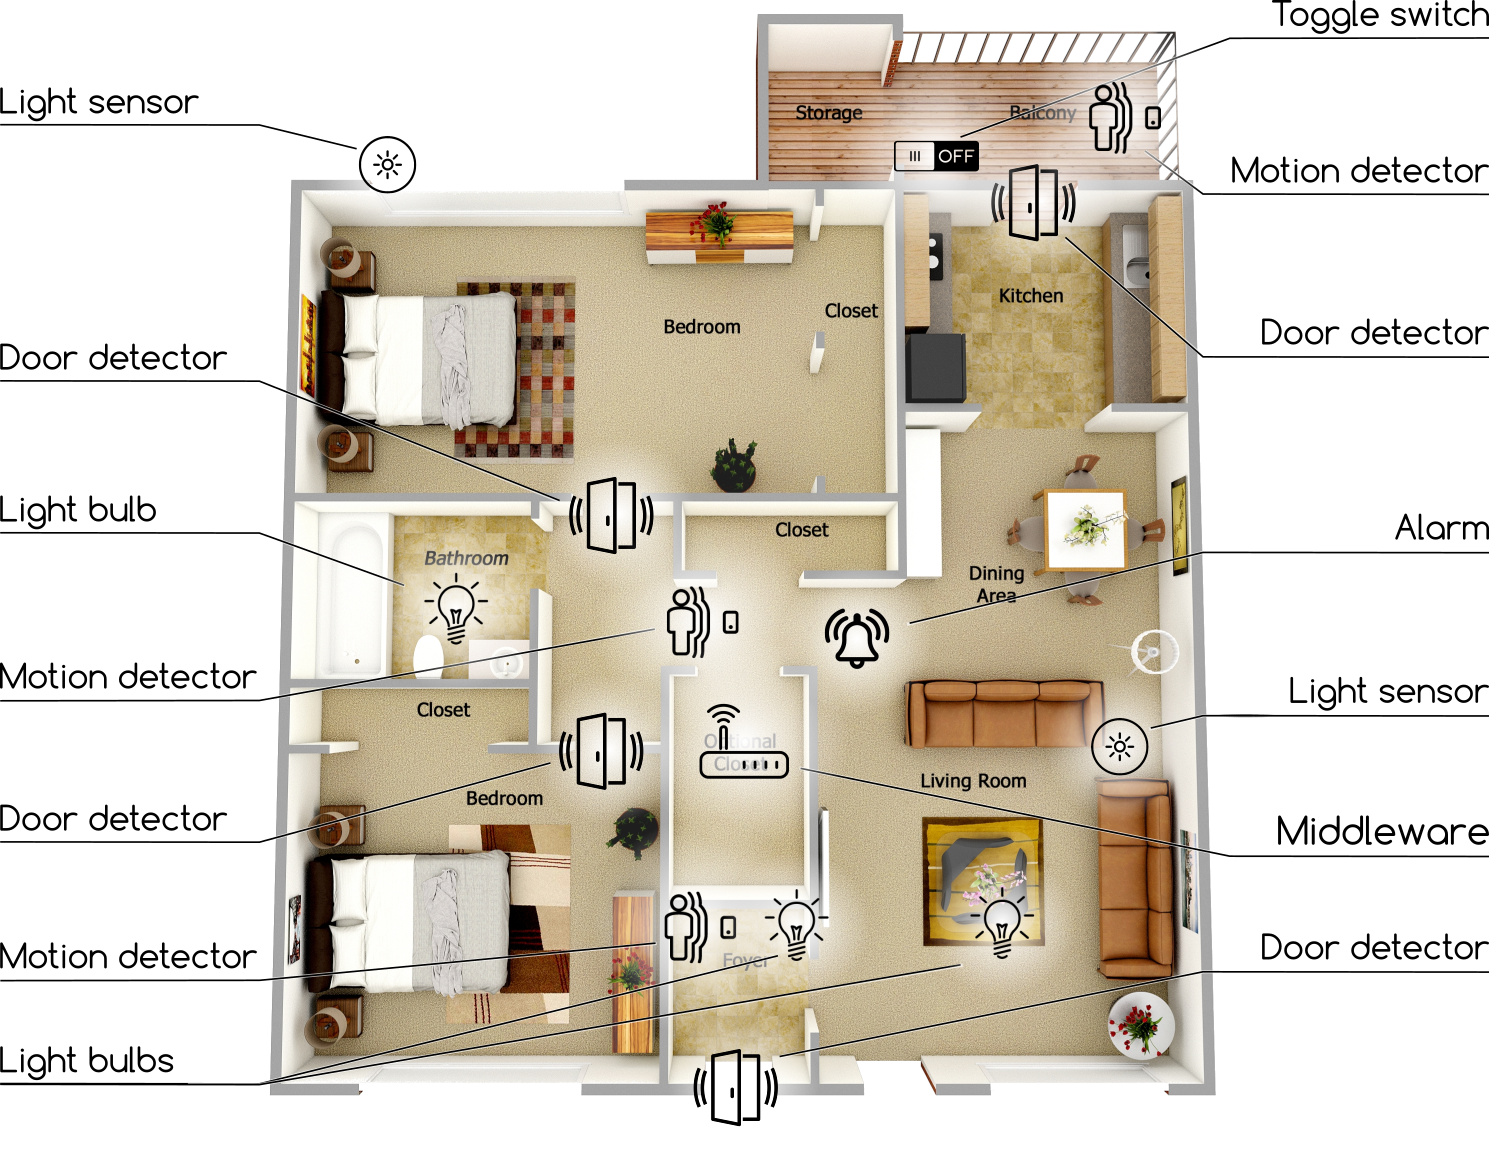
\includegraphics[width=.9\linewidth]{scenario.png}%
	\caption{Hypothetical Alice's \textit{smart-home} configuration of \IOT devices}%
	\label{fig:scenario}%
\end{figure}

Alice is interested in simple scenarios for her comfort and her little boy's security: she wants the entrance lights to automatically switch on to welcome her when she arrives home; 
%she likes her apartment to stay reasonably warm along the year; 
and since her boy often plays in the balcony, or sometimes wakes up at night and walks through the apartment, she needs to ensure he does not fall or injure himself.
Those scenarios seem already possible with the equipment she currently has: we will show how to implement them through a rule-based specification in Section \ref{sec:IoTDSL-BusinessRules}.

%This typical smart home configuration consists of light sensors and bulbs to handle the light in the apartment, motion and door detectors to verify the presence of persons, an alarm in case of emergency and a toggle switch on the balcony. Even if the amount of types of devices is rather limited, we can already highlight a set of features absolutely needed to describe the devices, network configuration and specify its dynamic aspects.


\section{Challenges}
\label{sec:Challenges}

\begin{description}
	\item[Capability Discovery] Providing the ability to drive interconnected devices assumes the capacity of automatically discovering devices' capabilities in a standardised and uniform way. Similar processes happened for other technologies: for example, an \textsc{Usb} device plugged into a computer automatically exposes its nature (e.g., a pointing or video device) and capabilities. This also requires a large ontology that classifies the many dimensions IoT devices are capable of (e.g., \cite{}).
	
	\item[Low-Level Event Reification] Furthermore, the events selected by the device constructors for operating one device could be radically different from what an end-user would expect to drive a particular solution: e.g., a heart rate monitor needs to scan pulsations every millisecond while what interests the user is the rate per minutes. An effective solution for defining high-level customised usage scenarios requires that a mapping between events perceived within a \textsc{Dsl} are bidirectionally mapped to low-level device events, or other artefacts that govern devices' functionalities. Symetrically, the open question of exposing low-level events to users can be useful for some scenarios, but critical in other situations. 
	
	\item[Protocol Interoperability] A domotic solution with heterogeneous devices would often integrate devices from various constructors, thus communicating through multiple communication protocols. In order to make them communicate efficiently, without forcing end-users to stick with one constructor that can dictate costs and restrictions without any control, a powerful \textsc{Dsl} should provide ways for interoperability over multiple communication protocols, without forcing end-users to understand the protocols' intricacies, version evolution, and restrictions.
	
	\item[Reactive Framework for \textsc{Bl}] 
	
	\item[Complex Event Processing (\textsc{Cep})] consists of deriving meaningful conclusions from a stream of events occuring within a system and of responding to them as quickly as possible. 
	%, by tracking and analysing them with various techniques, such as pattern detection, abstraction, filtering, relationship detection, and transformation.
	
	\item[Decentralisation Features] 
	
	\item[Non-Functional Properties] 
\end{description}

\subsection{Components for an \IOT Language}
\label{sec:Motivation-Components}

We argue that a good way of capturing the many variations of scenarios relying on a specific \IOT system deployed at home would consists in offering end users, i.e. home inhabitants like Alice, and technicians in charge of configuring such systems and effectively deploying them, a \DSL that provides at least the following components:

\begin{description}
	\item[Device Description] We need facility to make a precise inventory of the devices used in a specific deployment as well as the high-level capabilities of these devices, described in terms that are immediately understandable by end-users, as opposed to conveying technical details about how those devices precisely operate;
	
	\item[Network Description] A way to capture where each device is located and how it is possible to communicate with it, in order to receive or send data to it;
	
	\item[Dynamics] A way to describe the interactions wished by end-users, \textit{i.e.} how to leverage the functionalities of the devices to effectively realise one or several scenarios that are convenient for the end-users.  
\end{description}

Those components are obviously not sufficient to obtain a fully-fledged solution that becomes adaptable to any situation, but they still represent necessary steps to provide end-users the capacity to manipulate a collection of devices without relying on specific technologies. Defining such \DSLS should encompass a series of facilities dedicated to hide hardware- and protocol-related constraints, and high-level models of devices should somehow be easily \emph{transformable} and \emph{traceable} into concrete infrastructures with simulation and verification possibilities.


\section{IoTDSL}
\label{sec:IoTDSL}

Based on the challenges identified in Section~\ref{sec:Motivation}, we now introduce \IOTDSL, our \DSL devoted to facilitate the high-level manipulation of \IOT systems. At the heart of \IOTDSL are two governing principles. First, we promote a clean separation of concerns for all aspects the \DSL has to handle, by specifying one sublanguage for each concern. We believe this approach to be scalable, and to support independent evolutions of each concern without impacting the other aspects, since those aspects are composed through well-defined interfaces. Second, our \DSL relies on events, a natural paradigm for specifying various models of interactions that is widely used in embedded and critical systems, and where a clear separation between the system and its environment is performed, further empowering the separation of concerns. Despite its early stage of development, \IOTDSL shows its ability to capture the definition of small-scale \IOT systems appropriately.

Building a well-calibrated \DSL is known to be difficult and error-prone. It usually requires a broad expertise of the domain under consideration before a consensus emerges on the domain's key concepts and how to effectively represent them. Fortunately, \MDE technologies operated substantial breakthrough over the past decade, allowing language designers to define their own \DSL structures and user interfaces more easily. Adopting such a trend, we have built an early prototype for our \DSL under GeMoC \cite[\url{http://gemoc.org}]{bousse-16}, a \MDE framework that supports both visual and textual representations as concrete syntaxes and maintains a full synchronisation between them. Since we are at early development stage, only a textual syntax is currently available to modellers, but other syntaxes, even graphical ones, can be smoothly added thanks to \textit{GeMoc}.

To illustrate our proposal, we show how \IOTDSL is built by describing each sublanguage, following the \DSL components identified in Section \ref{sec:Motivation-Components}, and illustrate them by providing the full implementation for Alice's apartment as depicted in Section \ref{sec:Motivation-Scenarios}.

\begin{figure*}%
  \centering  
  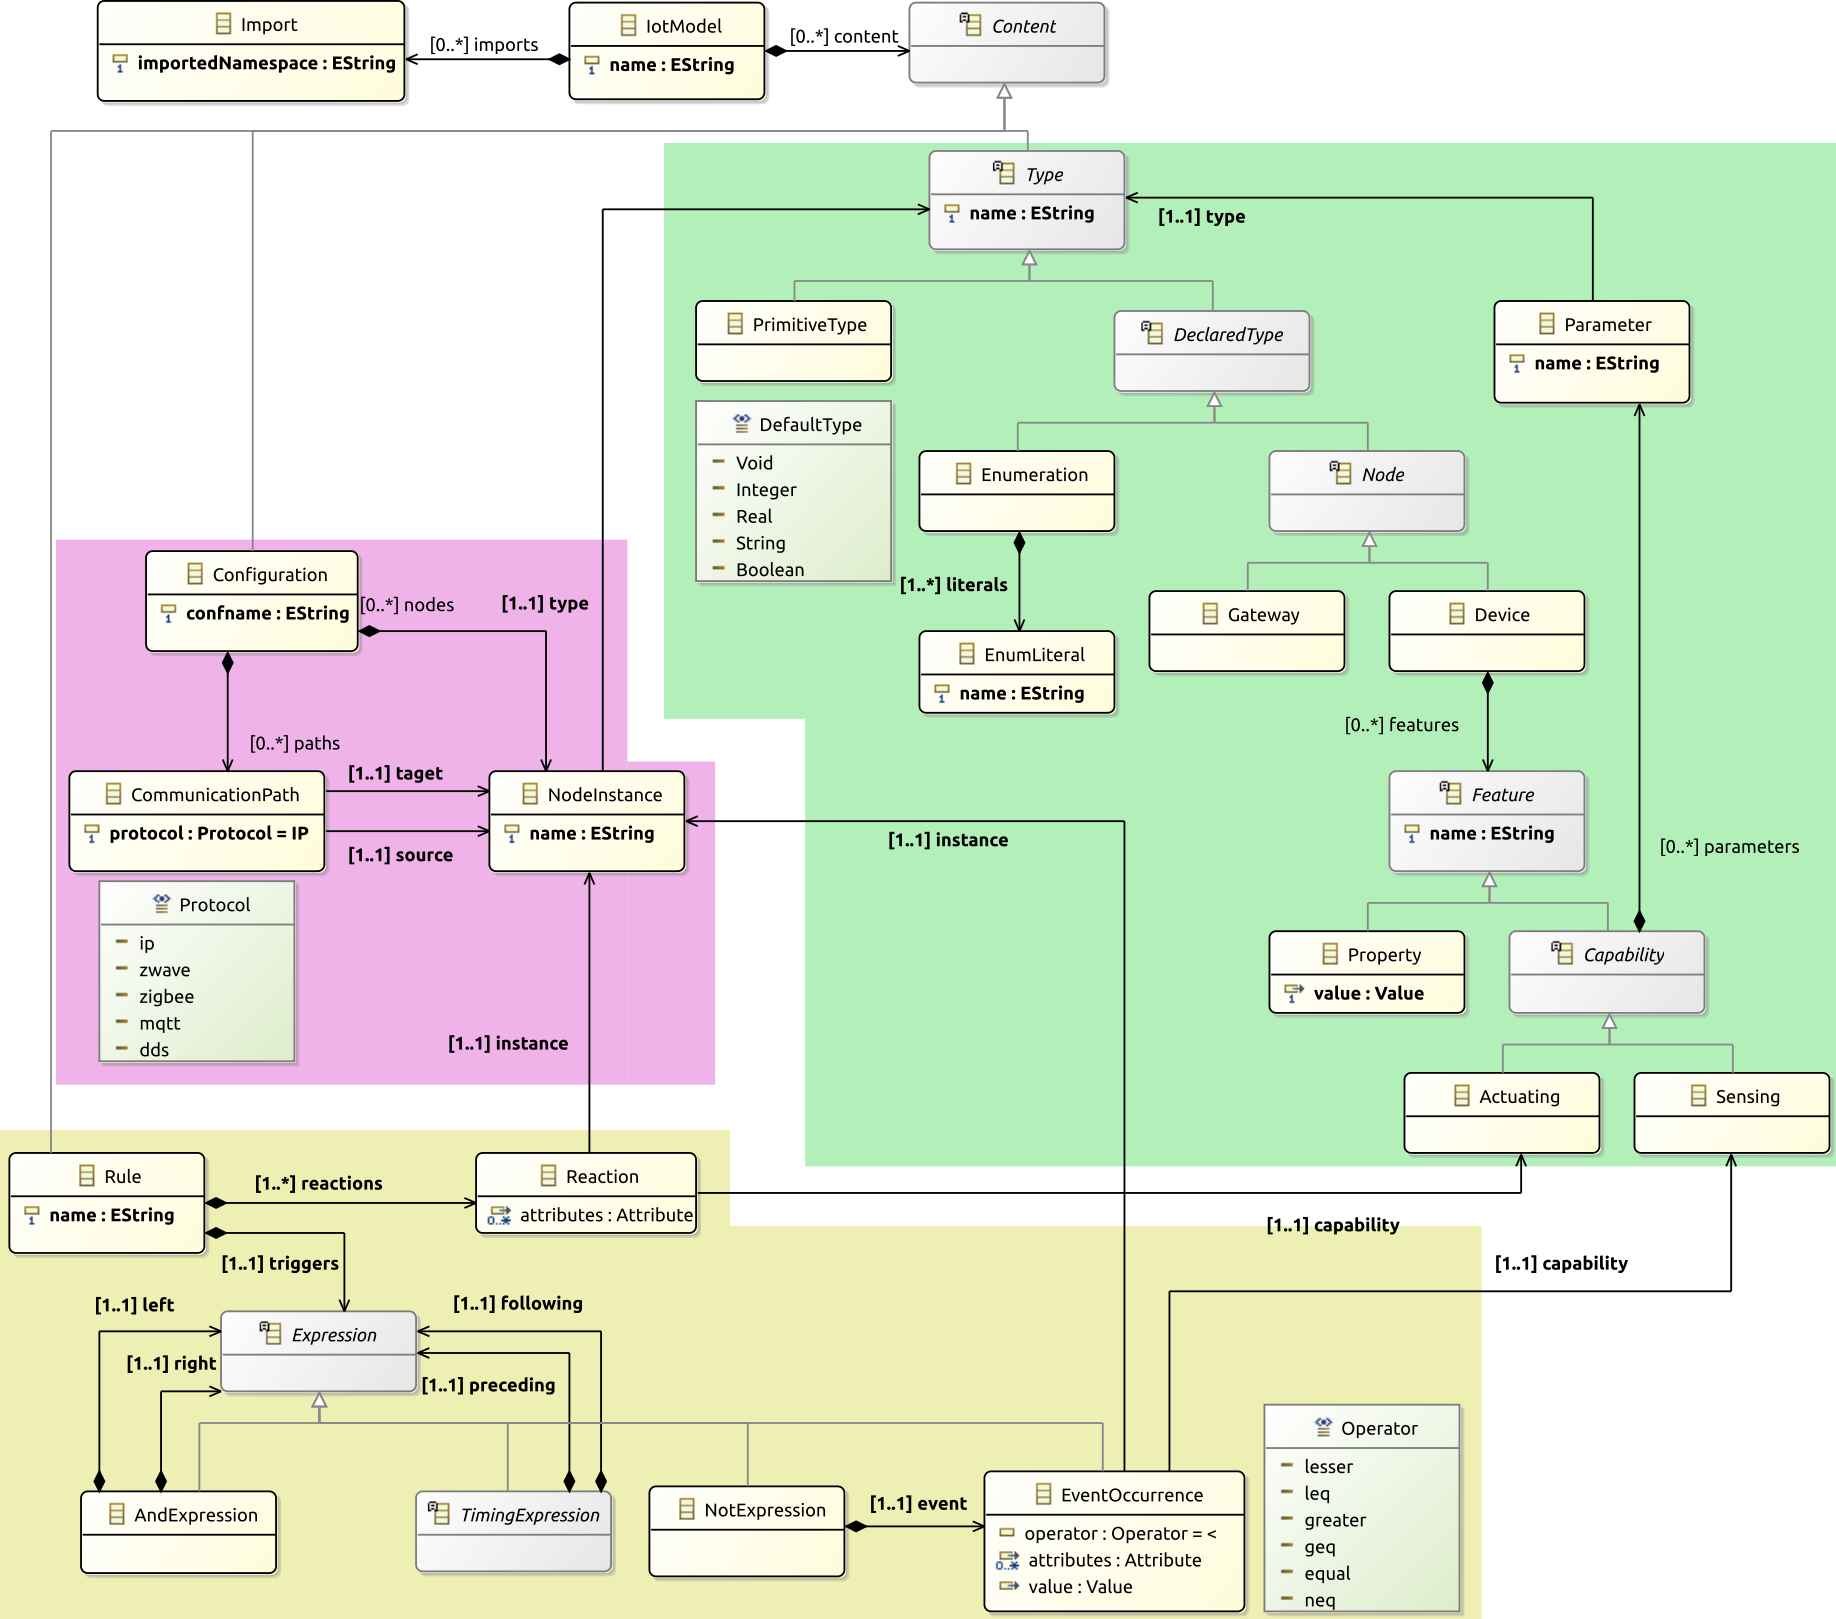
\includegraphics[width=.98\linewidth]{iotdsl-metamodel}%
  \caption{Metamodel of \IOTDSL, separated in three concerns: \emph{Type Definition} captures devices' capabilities (top-right green part), \emph{Network Configuration} details how device instances are connected to each others (middle-left purple part), \emph{Business Rules} defines the functionalities expected from the IoT installation (bottom yellow part).}%
  \label{fig:IoTDevice-MM}%
\end{figure*}

\subsection{Type Definition}
\label{sec:IoTDSL-TD}

The first task is to provide a description of which capabilities each device included in the \IOT system possess: how each device may provide information about the environment through a \emph{sensing} operation; and how it could react and influence it through \emph{actuations}. Our framework currently requires that an advanced user that is able to reason properly about how to effectively manipulate a device and extract the relevant information, but is flexible enough to accomodate automation in the future, so that information about devices could be automatically extracted from pre-existing devices databases (either from a knowledge database the \IOT system is connected to, or from a library of \emph{off-the-shelf devices}).

%In this section, we define \IOT devices' types, \textit{i.e.} which capabilities are available to the users in terms of getting information from the environment, \textit{a.k.a.} sensing, and operating on the environment, \textit{a.k.a} actuating. In our framework, type definitions either come from an advanced user who is able to reason properly about a particular device and extract the relevant information, or from a pre-existing devices database, either being a repository the system is connected to, or a library of \textit{devices-off-the-shelf}. 

\begin{figure*}%
  \centering  
  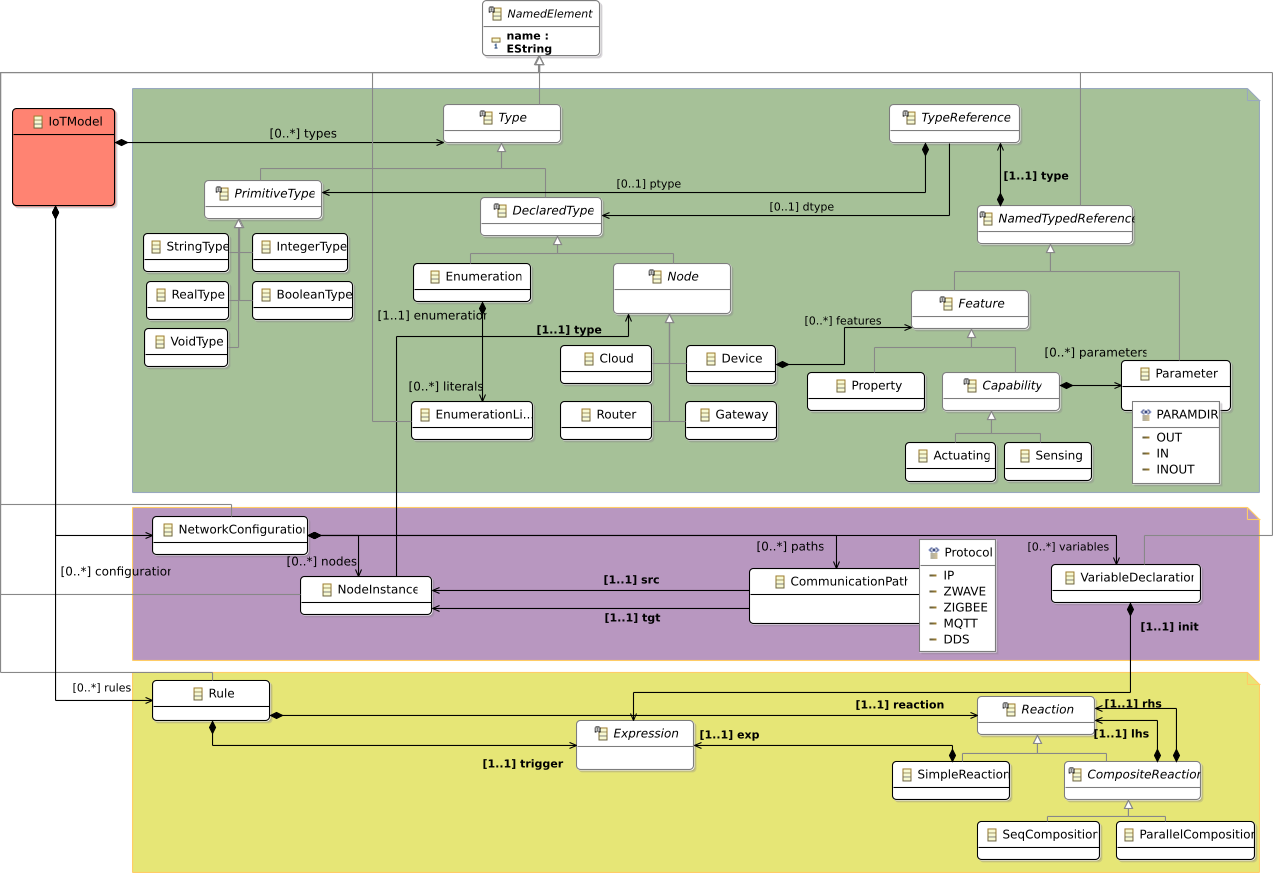
\includegraphics[width=.92\linewidth]{IoTDevice-MM.png}%
  \caption{Metamodel of \IOTDSL, separated in three concerns: \emph{Type Definition} captures devices' capabilities (top green part), \emph{Network Configuration} details how device instances are connected to each others (middle purple part), \emph{Business Rules} defines the functionalities expected from the IoT installation (bottom yellow part).}%
  \label{fig:IoTDevice-MM}%
\end{figure*}

The concepts dedicated to type definition are shown in Figure~\ref{fig:IoTDevice-MM} (green background). This part is similar to the notion of \textsf{Classifier} in \textsc{Mof}-like languages: a \textsf{Type} is either a \textsf{PrimitiveType}, or a user-defined \textsf{DeclaredType}. We distinguish between general \textsf{Gateway}s, which centralise information and processing, and \textsf{Node}s deployed in the environment and communicating with gateways, and which possess capabilities to interact with the environment. A \textsf{Capability} is basically a parameterised event that drives the node to either capture data from the environment, to act on it, or to perform both. This abstract view of an ``thing'' allows us to manipulate any device at a high abstraction level, exhibiting a clean and uniform interface for end-users based on device capabilities. Since \textsf{Node}s are \textsf{Type}s themselves, it remains possible to reference them as a parameter for the purpose of dynamic discovery across devices.

Listing~\ref{lis:RE-TypeDeclarations} illustrates how the devices in Figure~\ref{fig:scenario} are declared in \IOTDSL. Each device is introduced by the keyword \textsf{device}, possesses a name and lists capabilities that correspond to reporting events (\textsf{sensing}) or operating over the environment (\textsf{actuating}). 

\begin{table}
	\begin{minipage}[b]{.45\textwidth }%
		\begin{lstlisting}[language=iotdsl]	
gateway Middleware
device DoorDetector {
	sensing opened()
	sensing closed()
}
device MotionDetector {
	sensing moving()
}
device ToggleSwitch {
	sensing toggle()
}
		\end{lstlisting}
	\end{minipage}\hfill%
	\begin{minipage}[b]{.45\textwidth}
		\begin{lstlisting}[language=iotdsl, firstnumber=12]
		
device LightSensor {
	sensing light()
}
device LightBulb {
	actuating on()
	actuating off()
}	
device Alarm {
	actuating sound()
}
		\end{lstlisting}
	\end{minipage}
	\caption{Type declarations in \IOTDSL: capabilities as high-level events.}
	\label{lis:RE-TypeDeclarations}
\end{table}

Any IoT system should declare a special device, introduced with the keyword \textsf{gateway}, that centralises data from all devices connected to it, as we will show in Section \ref{sec:IoTDSL-NetworkConfiguration}. This device will be responsible of the event orchestration and will host the \CEP engine that embeds the implementation of the business rules. Also note that the above model is the \textit{user-defined} part of \IOTDSL. In the background, abstract events attached to all devices will need to be mapped to concrete low-level \textsc{Api}s events using a dedicated mapping language that is out of the scope of this paper.


\subsection{Network Configuration}
\label{sec:IoTDSL-NetworkConfiguration}

The configuration constructs of \IOTDSL are specified in the middle-left purple part of Figure~\ref{fig:IoTDevice-MM}. Since we use an architecture centralised around gateways, a network \textsf{Configuration} is a graph-like structure where vertices are \textsf{Gateway}s and \textsf{NodeInstance}s (so that instances may communicate with each others), while edges represent \textsf{CommunicationPath}s (or channels). Such paths define, among others, one or more protocols used to interact. We actually rely on existing platforms, such as OpenRemote (\url{http://www.openremote.org}) or SmartThings ({\url{https://www.smartthings.com}) to handle the intricate details of the protocols since such details are, from an end-user point of view, technical aspects rather than essential matters of the configuration itself. By knowing which protocols are used between each pair of devices, we can automatically perform data conversion in the proper format required by the protocols: most of those protocols are already implemented in \textit{General-Purpose Programming Languages} (\textsc{Gpl}s), like Java or C.

Listing~\ref{lis:RE-Network} shows an instantiation as well as the connection that conforms to the types given in Listing~\ref{lis:RE-TypeDeclarations} and the configuration presented in Figure~\ref{fig:scenario}.
	
	
\begin{table}
	\begin{minipage}[b]{.45\textwidth }%
		\begin{lstlisting}[language=iotdsl]	
configuration SmartHouse {
	node middle   		   : Middleware
	node alarm					 : Alarm
	node toggle          : ToggleSwitch
	node frontDoor			 : DoorDetector
	node parentDoor			 : DoorDetector
	node childDoor			 : DoorDetector
	node balconyDoor 		 : DoorDetector
	node outLight				 : LightSensor
	node livingLight		 : LightSensor
	node livingBulb			 : LightBulb
	node bathroomBulb    : LightBulb
	node foyerBulb       : LightBulb
	node balconyMotion	 : MotionDetector
	node foyerMotion  	 : MotionDetector
	node hallMotion	     : MotionDetector
		\end{lstlisting}
	\end{minipage}\hfill%
	\begin{minipage}[b]{.45\textwidth}
		\begin{lstlisting}[language=iotdsl, firstnumber=17]
	from alarm			   to middle via IP
	from frontDoor 	   to middle via IP
	from parentDoor    to middle via IP
	from childDoor     to middle via IP
	from balconyDoor   to middle via IP
	from outLight      to middle via IP
	from livingLight   to middle via IP
	from livingBulb    to middle via IP
	from bathroomBulb  to middle via IP
	from foyerBulb     to middle via IP
	from balconyMotion to middle via IP
	from foyerMotion   to middle via IP
	from hallMotion    to middle via IP
}
		\end{lstlisting}
		\vspace*{.3cm}
	\end{minipage}
	\caption{Network Configuration in \IOTDSL for our smart house.}
	\label{lis:RE-Network}
\end{table}
	
A specific device is considered as an instance of a defined type such that particular devices with the same set of capabilities may be distinguished via identifiable unique references. Communications are purely declarative and only mention the protocol type (introduced by the \texttt{\color{codeviolet}{\textbf{via}}} keyword). In our example, we simply decided to use an \textsf{IP} protocol for all bindings. Note that a similar mapping process that the one described at the end of Section~\ref{sec:IoTDSL-TD} is required to reify abstract connections between \textsf{NodeInstances} to physical ports and protocols, but again, these mapping statements are outside of the scope of this paper. 


\subsection{Business Rules}
\label{sec:IoTDSL-BusinessRules}

Business rules are the core of the manipulation of \IOT systems and compose the third part of \IOTDSL as detailed in the bottom yellow part of Figure~\ref{fig:IoTDevice-MM}. This last sub-language relies on an event-based framework that allows to specify a set of \textsf{Rule}s expressing the many functionalities an end-user wants to achieve in his/her concrete configuration. 

An \IOTDSL Business Rule is identified by the keyword \textsf{rule} followed by an unique identifier, and a body of the form << \texttt{\textbf{\color{codeviolet}{when}} trigger \textbf{\color{codeviolet}{do}} reaction} >>. Rules' \texttt{trigger}s are cyclically evaluated against the surrounding environment and specify the conditions under which the corresponding \texttt{reaction}s have to be performed to realise the end-users' scenarios. A \texttt{reaction} defines actuations on the \IOT system to send or require data of identified devices, or issues events that are internally used to synchronise rules. 

%must be triggered. Rules' \textsf{trigger}s are cyclically evaluated against the surrounding environment and a \textsf{reaction} defines a sequential or parallel combination of capabilities, enabling to sort actions by, or require data from some identifiable devices. Inside the \textsf{trigger}, users typically check events to evaluate their presences, but as we will see in the following examples, they are also able to check on their absence or returned values. A typical \textsf{reaction} may be to switch on all lights in a house, or only the ones of a certain type by sending new events.

Our approach is currently purely middleware-oriented: all rules are evaluated inside a single gateway that supposedly possesses enough processing power. We leave as future work the exploration of parallelisation techniques to support multiple gateways that communicate appropriately, or the possibility to decentralise parts of the computation into nodes with sufficient processing and power resources to optimise resource consumption and lighten communication exchanges. 

We now illustrate how the scenarios Alice is concerned about (cf. Section \ref{sec:Motivation-Scenarios}) can be translated into business rules in \IOTDSL with the devices' definitions detailed in Listings~\ref{lis:RE-TypeDeclarations} and \ref{lis:RE-Network}. 

\begin{description}[leftmargin=0cm]
	\item[Switching entrance lights on when coming in]  When Alice gets home (and thus opens the front door), she wants the lights to be automatically switched on in the foyer and in the living room.
	\begin{lstlisting}[language=iotdsl,
							label=lis:home-rule,
		caption=Rule to switch on the lights at home incoming]
rule SwitchLightsWhenEntering:
	when (foyerMotion.moving after frontDoor.opened) do {
		foyerBulb.on
		livingBulb.on
	}
	\end{lstlisting}
	This rule introduces what we call \emph{facilitators}, i.e. keywords that define an unspecified time window in which a sequence of events should be observed. This time window is system-specific and needs to be defined independently in configuration files independent of descriptions in \IOTDSL. In this case, the \inlineI{foyerMotion} should detect movement \emph{nearly after} the \inlineI{frontDoor} detects an opening. 
		
	Note that reactions are defined as a sequence that does not matter: the order in which the \inlineI{foyerBulb} and the \inlineI{livingBulb} switch on largely depends on the platform capacities, i.e. they can be actuated synchronously or sequentially (in which case, no guarantee is given that the definition order will be respected). At the abstraction level \IOTDSL operates, it is irrelevant since the end user wishes to see both switched on at some point, without having to consider low-level details that would enforce such behaviour.

	\item[Illuminate bathroom when children wake up at night] When Alice's little boy wakes up at night, she would like to have the light in the bathroom to be switched on to prevent him from falling or injuring himself. Analogously, she wants the light to be switched off when he gets back to sleep afterwards.
	\begin{lstlisting}[language=iotdsl,
							label=lis:night-rule,
		caption=Rules to switch on\//off lights in the corridor at night]
rule SwitchBathroomLightOnAtNight:	
	when (not livingLight.light and 
	 (hallMotion.moving after childDoor.opened)) do {
		bathroomBulb.on
	}

rule SwitchBathroomLightOffAtNight:	
	when (not hallMotion.moving within 3 min from childDoor.closed) do {
		bathroomBulb.off
	}
	\end{lstlisting}
	The rule \inlineI{SwitchBathroomLightOnAtNight} introduces a new keyword \inlineI{not}, which represents the \emph{absence} of a certain event type, here \inlineI{livingLight.light}. This is different than simply observing some events occuring. Note also that the second part of the rule trigger uses parenthesis to relate the facilitator \inlineI{after} to the closest event \inlineI{childDoor.open}, instead of spanning on the whole condition.

	The rule \inlineI{SwitchBathroomLightOffAtNight} presents a combination of negation with an explicit time window with the construct \inlineI{within ... from}: it indicates that no event of type \inlineI{movement} from the hall motion sensor should occur in a three-minute time window after observing the \inlineI{closed} event from the boy's door, in order to trigger the rule. \IOTDSL defines several useful time units to cope with simpler definitions (seconds, minutes, hours, or a combination of the three). 
	

	\item[Report unsupervised children on balcony] Alice considers that it is a critical situation if a child enters into the balcony without her knowledge, because of fall risks. To avoid that, she placed a switch button high enough that only an adult could press when accompanying a child outside. If the button is not pressed within 3 seconds after someone enters the balcony, an alarm should sound.
	\begin{lstlisting}[language=iotdsl,
							label=lis:balcony-rule,
		caption=Rules to sound the alarm in case of an unsupervised child on the balcony]
rule AlarmWhenChildOnBalcony:	
	when (not toggle.toggled within 5 sec from 
			(balconyMotion.moving after balconyDoor.opened)) do {
		alarm.sound
	}
	\end{lstlisting}
	This last rules states that once the balcony door has been opened and movements are detected on the balcony, the alarm should sound unless the toogle button is pressed in a five-second time window. This rule is similar to \inlineI{SwitchBathroomLightOffAtNight}, except that the baseline of the time window is here a composite event using a facilitator: once an opening followed by movements on the balcony is observed, we expect the toggle button to be pressed. 
\end{description}

To summarise, an end-user uses the Business Rules sublanguage to specify the scenarios of interest in the form of \inlineI!when (trigger) do {actuations}!: the \inlineI{trigger} condition specifies the event (non-) occurrence pattern under which the \inlineI{actuations} are performed, by using common boolean connectors as well as time windows to observe delayed events; whereas the \inlineI{actuations} are undeterministically performed independently to their definition order. 

From a qualitative point of view, adopting a rule-based language presents the advantage of mimicking the cognitive process of establishing a scenario, which should ease the adoption of \IOTDSL. However, we are conscious that this requires a further examination and actual validation with end-users that are not aware of the underlying \DSL mechanisms, but we believe that presenting a visual representation for rules and powerful analysis of rule activation could ease the adoption process and facilitate scenario definitions.







\section{Code Generation}
\label{sec:CG}

\subsection{TRex as \CEP engine}
\label{sec:CG-TRex}

To enable efficient event processing from distributed connected things, we rely on TRex, a powerful and highly optimised \CEP engine developed by Cugola and Margara~\cite{cugola-12}. TRex relies on Tesla \cite{Cugola-Margara:2010}, an entry language that is expressive enough to address most of the necessary patterns for capturing complex events definitions. As a consequence, the expression language used for \IOTDSL \textsc{triggers} is directly inspired from Tesla. This allows us to offer end-users the expressibility they need, while at the same time simplifying the translation of \IOTDSL rules into Tesla rules. 

TRex offers a queueing mechanism to overcome bursts of incoming events: when deploying the \IOT system on site, it becomes possible to customise the queue size, thus balancing between event loss and treatment latency. 

TRex is conveniently organised as a Client/Server architecture in a \textit{<<publish / subscribe>>} way, and relies on the Tesla language to define the necessary components: event \emph{notifications} (or \emph{occurrences}, or simply events); \emph{subscriptions} and \emph{rules}. TRex, as the \CEP engine, permanently receives event notifications from sources, and redistribute them to subscribers. 
An event notification is produced by a source and sent to the \CEP system, and is typed by an event type that possesses typed attributes: for example, \inlineT{Temp@100(location = ``Living'', value = 25.0)} defines a notification of type \inlineT{Temp} with two attributes and a timestamp (noted after the \inlineT{@}) that records the moment in time the notification is produced. A subscription by sinks (or, event consumers) is submitted to the \CEP system in order to receive notifications that things happened: for example, \inlineT{Subscribe(Temp, location = ``Living'' and value > 20)} indicates a subscription to \inlineT{Temp} notification that matches the filtering condition on its location and value. Tesla rules define complex events from simpler ones, which may emanate from actual sources, or be complex events defined by other rules, thus leading to a hierarchy of events. 

A rule has the following form:
\begin{lstlisting}[language=tesla, numbers=none]
	define CE(attr1 : Type1, ..., attrN : TypeN)
	from   Pattern
	where  attr1 := f1, ..., attrN := fN
\end{lstlisting}
Intuitively, a rule defines a complex event \inlineT{CE} together with its signature (i.e. an ordered list of typed attributes) that issues \inlineT{CE} notifications whenever the \inlineT{Pattern} is matched, assigning values to \inlineT{CE} attributes from the functions defined in the \inlineT{where} clause (that may depend on elements of the \inlineT{Pattern}). Valid patterns include event \emph{occurrences} that filter attribute values (e.g., \inlineT{from Temp.val > 20}), event \emph{compositions} that combine events together with boolean operators or time windows (e.g., \inlineT{from Rain and Temp.val > 20 within 5 min from Smoke}, indicating that a temperature reading above 20°C should occur within five minutes from a \inlineT{Smoke} notification, while raining); event \emph{negation} (e.g., \inlineT{from not Rain between Temp and Smoke}, indicating that it should not rain between an elevated temperature reading and a smoke notification). Tesla proposes more powerful patterns like aggregation and iterations, but we will not use them in our examples.
Note that the server is interactive so that clients can (un-)subscribe while the engine is running and rules may be added or deleted at runtime without affecting the overall infrastructure. 

From the perspective of \IOTDSL, TRex offers several benefits as a \CEP engine. TRex is powerful enough to handle typical \IOT scenarios like the one described in Section \ref{sec:Motivation}, thanks to the expressive power of Tesla. It adopts a decentralised architecture that directly reflects our design choices, and supports distributed processing of events to reduce the cost of communication and to optimise resource usage. It is developed in C, so it is even suitable for \textit{small form factor} middlewares. Finally, on top of an \textsc{API} written in C, Java libraries have been developed on which we rely to generate devices' simulation code.

\subsection{General Architecture}
\label{sec:CG-Architecture}

Our proposal relies on a middleware that embeds a \CEP engine for handling event processing, as depicted in Figure \ref{fig:Architecture}. Our tool offers a simulation mode, where devices are simulated as software components mimicking their actual execution, thus allowing to test \IOT scenarios without physical devices.

\begin{figure}%
	\centering  
	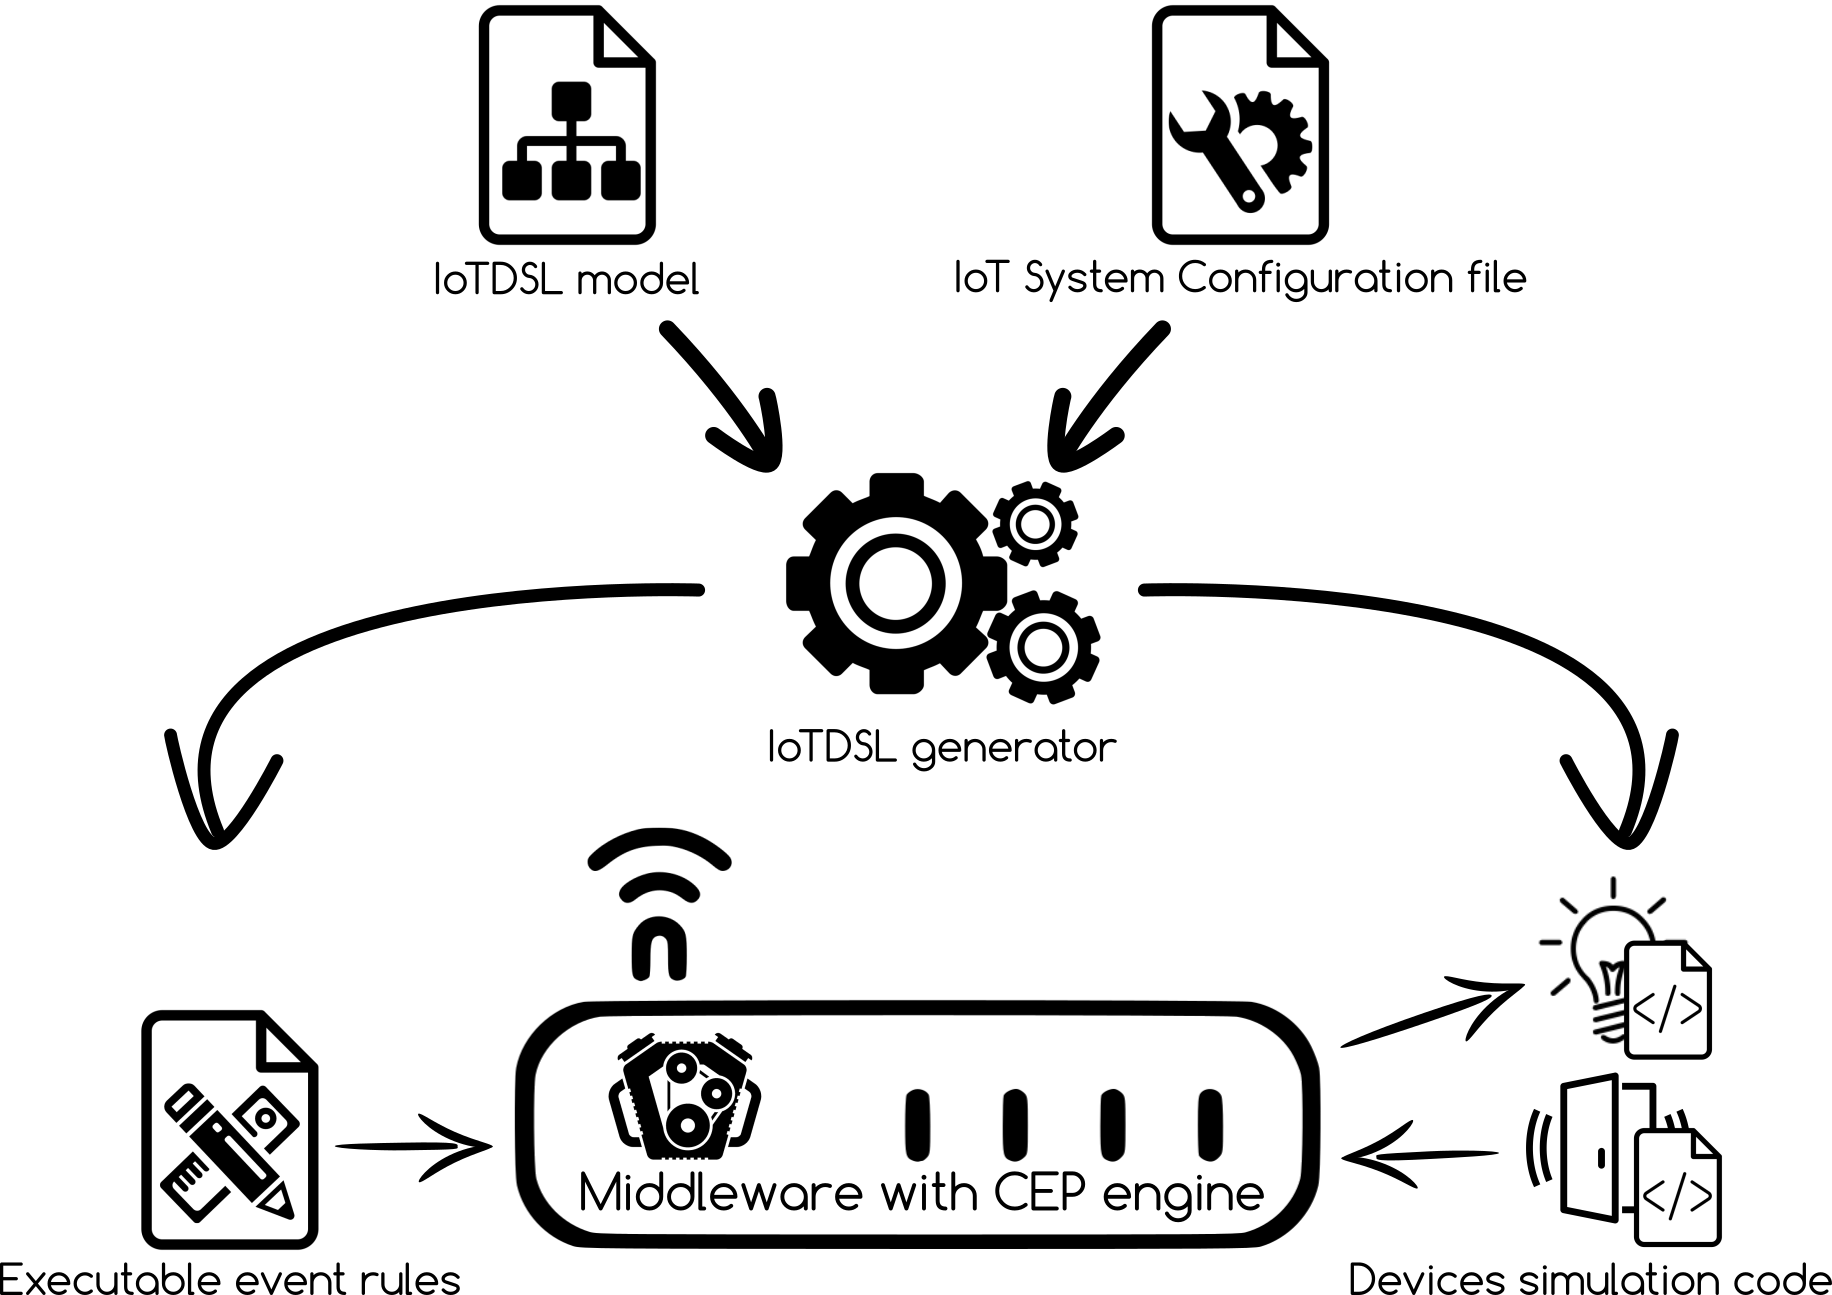
\includegraphics[width=.9\linewidth]{gen-archi.png}%
	\caption{General architecture of \IOTDSL framework}%
	\label{fig:Architecture}%
\end{figure}

The central element is the automatic code generator process: it produces executable code from \IOTDSL models and configuration files that define platform-specific details on the execution timing of devices (that the technicians set once and for all), and, for the purpose of our prototype, simulation code used to emulate the behaviour of the devices. The executable code is deployed into the \CEP engine running on a middleware, which reuses in simulation mode the simulation code for communicating with the (abstract) devices. 

%From \IOTDSL models, the generator will create a set of files that gather, on the one side, all rules as executable complex events and on the other side, a set of simulation code used to emulate the devices' behaviours. The event rules will be deployed in a \CEP engine running on a middleware and the individual simulation files will be used to test the whole infrastructure.

We are currently investigating how business rules could be broken down into smaller clusters that could be deployed directly into devices, assuming they present sufficient battery and computing power. When addressing non-functional properties of devices, we envision the possibility of expressing technical specifications relative to the energy consumption and computation capabilities of devices in a separate file that \IOTDSL would take into consideration for identifying distributable rules.

%As we already mentioned, at present time the rules are all gathered and managed by a centralised entity where the simulation files are each emulating a single device. We are currently investigating how all business rules can be split into smaller chunks to be run on devices themselves when those objects have sufficient battery and CPU power. As we are developing the non-functional properties for \IOTDSL type and mapping definitions, those characteristics will be expressible in the form of technical specifications for devices and thus powerful equipments that are meeting some minimum requirements will be identified as deployment targets for distributed \CEP engines. 
\subsection{Compiling \IOTDSL Rules}
\label{sec:CG-Compilation}

We now describe how we obtain the final code deployed into the gateway using TRex, and illustrate our compilation scheme on the Business Rules of Section \ref{sec:IoTDSL-BusinessRules}.

In \IOTDSL, a Business Rule has the following general form: \inlineI{rule R: when (trigger) do reaction}. The scheme for producing Tesla code relies on a three-step process:
\begin{enumerate}
	\item For traceability purposes, we map each rule name \inlineI{R} to the resulting Tesla rule(s), to be able to trace in the future analysis results directly back to \IOTDSL rules.
	
	\item The second step requires a preliminary task: since Tesla does not handle instances (in the form of our dot-like notation for events), we need to add a predefined attribute \inlineT{E(_inst : Instance)} to each event \inlineI{E} used in \IOTDSL Business Rules, and link the type \inlineI{Instance} to simple strings; unicity of instance names is ensured by \IOTDSL while checking Network Configurations. The rest of the second step depends on the nature of the \inlineI{reaction}:
	\begin{itemize}
		\item If it is not a composite, i.e. the rule consists of only one actuation of the form \inlineI{inst.actuation(<param1, ..., paramN>)}, we translate it in a simple rule of the form
		\begin{lstlisting}[language=tesla, numbers=none]
	define actuation(param1, ..., paramN)
	from   transformedTrigger
	where  param1 := f1, ..., paramN := fN
		\end{lstlisting}
		where the actuation parameters are computed in the \inlineT{where} line, and the \inlineI{trigger} condition is transformed into \inlineT{transformedTrigger} with the process in Step 3.
		
		\item If the \inlineI{reaction} is composite, i.e. it consists of several actions \inlineI{a1}, \ldots, \inlineI{aN}, we issue $n+1$ Tesla rules: one rule for each actuation \inlineI{aI}, and one additional rule to bind things together.
		\begin{center}
			\begin{lstlisting}[language=tesla, numbers=none]
	define R(Rparam1, ..., RparamM)
	from   transformedTrigger
	where  Rparam1 := g1, ..., RparamM := gn
	...
	define aI(AIparam1, ..., AIparamN)
	from   R(Rparam1, ..., RparamM)
	where  AIparam1 := f1, ..., AIparamN := fn
	...
			\end{lstlisting}
		\end{center}
		When the event pattern for the rule \inlineI{R} is detected, the first rule issues the complex event \inlineT{R}, which is immediately produced by the \CEP engine to trigger the subsequent rules. This way, all actuations are processed at the same time, leaving the platform handling how to effectively enforce the actuations. Note that in the additional Tesla rule \inlineT{R}, no \inlineT{_inst} parameter appears (as it is not needed), but all parameters necessary to the $n$ actuations are part of event \inlineT{R}'s signature, so that functions \inlineT{f1}, ..., \inlineT{fN} rematches the parameters of each actuation (\inlineI{aIparamK}) correctly from \inlineT{R}'s parameters.
	\end{itemize}
	\item It then remains to compute the \inlineT{transformedTrigger} appearing in Tesla rules, which depends on whether facilitators (like \inlineI{after} or \inlineI{before}) have been used. In the absence of facilitators, the transformation is straigthforward since the same expressions are natively available in Tesla. Otherwise, we rely on an external configuration file that describe the expected latency delays specific to devices and their communication paths, to translate such triggers into appropriate time windows. Producing this file is not the responsibility of the end-user, since it rather leverages knowledge pertaining to the \IOT system installation and deployment. 
\end{enumerate}

Let us now apply this compilation scheme to the three Business Rules described in Section \ref{sec:IoTDSL-BusinessRules}. Rule \inlineI{SwitchBathroomLightOffAtNight} is the simplest one: it contains only one actuation, and its triggers has a regular Tesla time window expression. Applying our compilation scheme results in the following Tesla rule:
\begin{lstlisting}[language=tesla, numbers=none]
	define Off(_inst : Instance)
	from   not Movement(_inst = hallMotion) within 3 min from Closed(_inst = childDoor)
	where  _inst = bathroomBulb
\end{lstlisting}
Note that all event names are capitalised to cope with Tesla entry language, and that the \inlineT{from} clause only binds the \inlineT{_inst} attributes to their respective instances in the source \IOTDSL rule. 

Rule \inlineI{SwitchLightsWhenEntering} is a good illustration of \IOTDSL rules with multiple actuations. Applying the compilation scheme results in three rules, one for each actuation, and an additional one that glues things together. 
\begin{lstlisting}[language=tesla, numbers=none]
	define SwitchLightsWhenEntering
	from   Moving(_inst = foyerMotion) within 10 sec from Opened(_inst = frontDoor)

	define On(_inst : Instance)
	from   SwitchLightsWhenEntering
	where  _inst = foyerBulb
	
	define On(_inst : Instance)
	from   SwitchLightsWhenEntering
	where  _inst = livingBulb
\end{lstlisting}
The additional rule defining the \inlineT{SwitchLightsWhenEntering} event does not define an \inlineT{_inst} attribute, and converts the event facilitator \inlineI{after} into a time window from a predefined value (here, 10 seconds). The two other rules originate from the actuators that have the particularity to activate the same event on two different devices (\inlineI{foyerBulb} and \inlineI{livingBulb}): this results in the same rule with different bindings for \inlineT{_inst}.

Rule \inlineI{SwitchBathroomLightOnAtNight} is the most complicated, since it combines negation outside a time window. Applying the compilation scheme results in only one rule, since there is only one actuation, but the trigger condition is more complicated that the first rule. Since Tesla does not support negation operators outside of time windows, we need to integrate it inside one. Intuitively, the starting point of this scenario is the opening of the door room: at this point, the bathroom light should be switch on if movement is detected shortly after and there is currently no light in the living. Such trigger patterns are detected and refactored as follows: 
\begin{lstlisting}[language=tesla, numbers=none]
	define On(_inst : Instance)
	from   (Light(_inst = livingLight) within  2 sec from Opened(_inst = childDoor)) and 
			   (Moving(_inst = hallMotion) within 10 sec from Opened(_inst = childDoor))
	where  _inst = bathroomBulb
\end{lstlisting}




\section{Discussion \& Remaining Challenges}
\label{sec:Discussion}

The \IOTDSL framework has been designed to empower non-experts with facilities regarding the requirements of \textit{smart home} \IOT solutions. Coupled to \IOT devices and network specifications, the framework offers a rule-based language compilable into a concrete \CEP infrastructure in charge of the event orchestration. \IOTDSL users are then able to describe their own configurations and needs in terms of conditional events and reactions to the manifestation of such conditions.

Tracing back to the features and challenges identified in Section~\ref{sec:Motivation-Challenges}, \IOTDSL currently covers most of these aspects. We created a description language that captures devices capabilities at a high-level of abstraction, describing them as entities that produce and consume (typed) events, relieving end users from acquiring the low-level knowledge to manipulate them. Based on these specifications, users become able to represent smart home configurations easily by describing links between devices and declaring which protocols are used for communication from a set of predefined, widely used protocols. Device interactions are simply expressed as conditions triggering other events that would react on the environment, inducing physical actions on the real world. These three sublanguages defined in \IOTDSL cover the identified language components identified as necessary for any \DSL dedicated to \IOT systems.

%We created a layered description language where type of devices can be described at a high level of abstraction, without requiring knowledge in a particular technology. Objects are simply described in terms of producing and consuming (typed) events. From these specifications, modellers are able to represent \textit{smart home} configurations by linking devices to each other with a predefined set of abstract communication protocols. Interactions between multiple devices are then simply  expressed as conditions triggering other events. Those three sub-languages of \IOTDSL just cover the three identified needed features of a \DSL for \IOT.

Based on the literature, we also identified in Section \ref{sec:Motivation-Challenges} seven important challenges an \IOT modelling solution should tackle. At the current development stage, \IOTDSL fully addresses the following challenges. \IOTDSL sees devices through their high-level capabilities, which basically corresponds to an ontological device description: it describes the \emph{interface} of devices in a general way, thus facilitating \emph{Capability Discovery} as it becomes available. By separating device descriptions from how they are connected to each others, \IOTDSL empowers \emph{Reusability} of devices through different \IOT systems; furthermore, since partial configurations could be easily defined and imported in \IOTDSL, partial definitions and behavioural specifications could also be shared between various instalments. 

We notably rely on a powerful \CEP engine to handle event orchestrations and deliver physical actions through the system. Our framework processes abstract business rules and transforms them automatically into executable code, and produces sample code for simulation purposes. The \emph{scalability} issue is almost exclusively concentrated on the device intercommunication and the rule processing, making scalability issues rely almost completely on the \CEP engine. TRex, the engine we have chosen, already offers parallelisation mechanisms that we will leverage to divide monolithic solutions into smaller entities that would collaborate, assuming an \IOT system becomes too large to handle, so that part of the business rules could be deployed on distinct parts of the system to minimise the middleware workload. In turn, these could generate even more events through the network and result in saturating it with data transmissions: an appropriate tradeoff needs to be found between having more one-to-one communications, or grouping more logics inside one node.

There is however three other challenges that we scarcely target with \IOTDSL, even if they are partially encompassed in some way, mostly because they represent orthogonal aspects or concerns that comes after the domain targeted by our language. \IOTDSL targets the manipulation of device \emph{interactions}, but already provides, through \CEP, a limited paradigm for \emph{Data Manipulation} that scales. However, as usual, a dedicated \DSL could be more relevant since the operations required for such operations are somehow different. An interesting discussion would then to identify the interface needed to exchange information between data retrieved from device interactions and data processed offline with higher processing capabilities. For now, \IOTDSL hides the intricacies of \emph{protocol communication interoperability} by implementing simple connectors to each protocol we handle, and reusing existing infrastructures for protocols that we do not handle natively. However, it could be interesting to propose a generic infrastructure for protocol communication by separating the transport layer from the message representation. This is a specific expertise domain on its own that we will tackle later. For \IOTDSL to handle \emph{non-functional properties}, we first need to have precise description of the devices hardware properties, which is an active research domain on its own. From that, we could integrate information that would guide the automatic code generation process to specialise the code to either decentralise parts of the processing activities, or ensure better performance, or integrate best practices for security.

%\begin{description}
	%\item[Capability Discovery] \IOTDSL \textsl{capabilities} have been designed to enable dynamic discovery of devices \textit{interfaces} as a \textsl{capability} can handle devices as parameters.
	%
	%\item[Reusability] By separating devices' descriptions to network configurations, \IOTDSL empowers reusability of devices in different \IOT systems. Furthermore, as partial \IOTDSL models can be imported into other models, partial definition of networks as well as behavioural specifications can be reused throughout models.
	%
	%\item[Complex Event Processing] \CEP is the core of \IOTDSL by which the whole events orchestration is handled. Abstract business rules are automatically transformed into a runnable infrastructure and sample code is also generated by the framework for simulation purposes. We notably rely on a powerful \CEP engine that will allow us to even decentralise the middleware code into collaborating nodes in future development of the framework.	
	%
	%\item[Scalability] As we rely on \CEP for device communication, almost the whole scalability issue is on the \CEP engine's hand. But, as we have chosen our infrastructure carefully, current monolithic solution is dividable into smaller entities that will collaborate if an \IOT network becomes large, such that some (set of) business rules will be deployed on distinct entities, minimising the work load on the middleware, even needing no middleware at all and working in a fully-decentralised way.
	%
	%\item[Data Management] To cope with an increase of exchanged data, prioritisation and decentralisation policies can be handled by our framework. On the one hand, thanks to configuration possibilities of TRex, events retention policies may be configured. On the other hand, again because TRex supports distributed evaluation of events, the workload may be scattered on the whole network. However, replicating \CEP-capable nodes may produce more events and saturate the network with data transmissions, so an appropriate trade-off must be found between having more \textit{one-to-one} communications or grouping more logic inside one node.
	%
%\end{description}

%However, we scarcely focus on the remaining two challenges, even if they are partially encompassed in current language.

%\begin{description}
	%\item[Protocol Interoperability] Concrete connections of \textit{things} is not addressed at current stage of development. Mapping rules between abstract devices definitions and concrete specifications of objects are under investigation. Furthermore, as a fully \MDE approach, \IOTDSL should provide generation capabilities of partial \textit{glue} code to map between tangible objects and our \CEP middleware.
%
	%\item[Non-Functional Properties] As for communication-specific features, more general non-functional properties should be expressible in \IOTDSL, especially as we deal with high-level user requirements. This essential aspect is also under investigation to empower modellers with semantic refinements at the typing level and also at the technical mapping level we are currently considering.
%\end{description}
\section{Related Work}
\label{sec:RW}

A series of overviews have been recently conducted on several aspects of \IOT. In \cite{alfuqaha-15,xu-14a}, the authors reviewed the applications, protocols and technologies used in the distinct \IOT layers, while \cite{singh-14,gubbi-13} focused on architectural aspects and \cite{tan-10,xu-14b} reviewed security ones. Most of these contributions identify a number of challenges crossing the application domain of a \DSL for \IOT, from which we identified the most relevant ones to our contribution in Section~\ref{sec:Motivation} and to which we confront our framework in Section~\ref{sec:Discussion}.

Capturing variations of a domain with explicit constructs close to the domain concepts resides at the essence of \DSLS. In that regard, many \DSLS were proposed for various purposes in the \IOT stack. \textsc{Chariot}~\cite{pradhan-15} addresses Cyber-Physical Systems by providing a component model that clearly distinguishes between communication and computation, while ensuring resilience features in highly reconfigurable systems. In~\cite{brandtzaeg-12} is presented a \DSL aimed at facilitating the deployment of applications, based on a component model of the environment used to locate the architecture nodes where business logic can be leveraged. \textsc{Alph}~\cite{munnelly-08} is a \DSL for ubiquitous healthcare that focuses on three concerns: mobility, by helping users to manage frequent devices disconnections; context-awareness to adapt application behaviour to environmental changes; and infrastructure, for managing the heterogeneity of communication protocols. Midgar~\cite{garcia-14} offers a visual interface to support end-users in controlling interconnected devices and generate the glue application making these devices interoperate. In~\cite{salihbegovic-15}, the authors present a visual \DSL for capturing the features and intercommunications of devices distributed in various application domains spanning from smart homes to patient monitoring. These contributions target different application domains at different abstraction levels, but possess every key features we identified in Section~\ref{sec:Motivation} in a more or less explicit way. Since \IOTDSL targets end-users with no prior knowledge in programming, we contrast with these contributions by offering a more intuitive, declarative style for expressing the system's dynamics through semantics rules that are compilable into a runnable \CEP engine.

ThingML~\cite{harrand-16} is the closest contribution to our \DSL: it uses a similar device description with messages and communication ports attached to devices, but describes the dynamics of devices and systems through state machines, which appear to be more obscure for end-users. However, the conceptual drawbacks are similar in both paradigms: state machines need to be deterministic on their transitions, while rules have to avoid multiple concurrent firing to avoid executing several rules at the same time. 

Other approaches, \textit{e.g.}~\cite{bhandari-13,cheng-16}, relying on the \textit{Event Condition Action} (ECA) paradigm, share a similar view for \IOT devices orchestration through \CEP, though not having the same expressiveness for devices' definition as we propose, especially with time frames and event compositions. In~\cite{shimokura-07}, the authors add \textit{pre-} and \textit{post-conditions} to ECA rules but they still do not address time frames constraints.

All previous contributions take advantages of \MDE technologies and tools. More general \MDE framework like GeMoC~\cite{bousse-16} or ThingML allow to specialise the description of interconnected devices, for example to describe Arduino systems specifically in ArduinoML~\cite{mosser-14}. On contrary, \IOTDSL framework concentrates on generating executable rules from user-defined requirements.
\section{Conclusion and Future Work}
\label{sec:Conclusion}

In this paper, based on recent research, we summarised the needed features as well as major challenges for the adoption of a specific language for \IOT systems. We introduced \IOTDSL, a domain specific language, designed to tackle those various challenges, \textit{e.g.} in terms of capability discovery, event processing or interoperability. In \IOTDSL, devices are described in a common \textit{Classifier} - \textit{Type} - \textit{Instance} layered specification that allows modellers to easily distinguish between typing and running instances concepts. A second benefit of that separation is the ability to create reusable \textit{libraries} of conceptual components, so \IOT devices by extension. By raising the abstraction level and hiding technical constraints to end-users, \IOTDSL is designed to serve as a handy modelling mean for them. Moreover, by abstracting the communication complexity into dedicated modelling construct, it is aimed to facilitate future evolution and re-configuration of existing solutions, since device descriptions may be retrieved from a centralized gateway.

Behavioural specifications are key aspects in \IOTDSL. We decided to rely on event-based \textit{rules} instead of state machines for their conciseness and readability, though rules may be converted to state machines automatically. Together with high-level \textit{operations} descriptions, they offer a more concise mean to describe dynamic aspects of \IOT configurations, without loosing formal model verification capabilities.

However, the prototype language is at early development stage and some features are currently missing or under development. First, the expression language must be validated on a real world examples and the mapping layer in charge of reconciling the abstract definitions and the technological APIs. Second, the complex composition of rules must be further investigated. Last, we plan to investigate on logic migration possibilities from the gateways to nodes with sufficient capacity. 
%\vfill
\bibliographystyle{apalike}

{\small \bibliography{./MODELSWARD2017.bib}}


\end{document}